% MATH 578 HW4
% LUKE WUKMER

\documentclass[10pt]{article}

% note: some of these are extremely useful and i don't remember why :o
%\usepackage{savetrees} % disable custom geometry stuff if you do this
\usepackage{titling}    % contol over title & stuff
\usepackage{amsmath, amsthm, amssymb, amsfonts}
\usepackage{amsxtra, amscd, geometry, graphicx}
\usepackage{endnotes}
\usepackage{cancel}
\usepackage{wrapfig}    %inline figs
\usepackage{bm} %allows fancy stuff like bold greek in math mode
\usepackage{alltt}
\usepackage{enumerate} %more/easier control over lists, also see enumitem
%\usepackage[all,cmtip]{xypic}
\usepackage{mathrsfs}
\usepackage{listings} % code with syntax highlighting etc
\usepackage{caption}
\usepackage[raggedright]{sidecap} % side captions
\usepackage{tabu}     % more customizable tables
%\usepackage{subfigure}
%\usepackage{subcaption}
%\usepackage[pdftex]{hyperref}
%\usepackage[dvips,bookmarks,bookmarksopen,backref,colorlinks,linkcolor={blue},citecolor={blue},urlcolor={blue}](hyperref}

\graphicspath{ {./figs/} }

\usepackage{color}


\definecolor{mygreen}{rgb}{0,0.6,0}
\definecolor{mygray}{rgb}{0.5,0.5,0.5}
\definecolor{mymauve}{rgb}{0.58,0,0.82}

\lstset{ %
basicstyle=\footnotesize,        % the size of the fonts that are used for the code
%breakatwhitespace=false,         % sets if automatic breaks should only happen at whitespace
breaklines=false,                 % sets automatic line breaking
captionpos=t,                    % sets the caption-position to bottom
commentstyle=\color{mygray},    % comment styleh
%  deletekeywords={...},            % if you want to delete keywords from the given language
%  escapeinside={\%*}{*)},          % if you want to add LaTeX within your code
%  extendedchars=true,              % lets you use non-ASCII characters; for 8-bits encodings only, does not work with UTF-8
frame=single,                      % adds a frame around the code
%keepspaces=false,                 % keeps spaces in text, useful for keeping indentation of code (possibly needs columns=flexible)
% columns=flexible,
  keywordstyle=\color{blue},       % keyword style
  language=Python,                 % the language of the code
%  otherkeywords={*,...},           % if you want to add more keywords to the set
%  numbers=left,                    % where to put the line-numbers; possible values are (none, left, right)
%  numbersep=5pt,                   % how far the line-numbers are from the code
%numberstyle=\tiny\color{mygray}, % the style that is used for the line-numbers
%  rulecolor=\color{black},         % if not set, the frame-color may be changed on line-breaks within not-black text (e.g. comments (green here))
showspaces=false,                % show spaces everywhere adding particular underscores; it overrides 'showstringspaces'
showstringspaces=false,          % underline spaces within strings only
%  showtabs=false,                  % show tabs within strings adding particular underscores
%  stepnumber=2,                    % the step between two line-numbers. If it's 1, each line will be numbered
  stringstyle=\color{mymauve},     % string literal style
%  tabsize=2,                      % sets default tabsize to 2 spaces
title=\lstname                   % show the filename of files included with \lstinputlisting; also try caption instead of title
}
% change up the fonts (pick one only)
%\usepackage{times}%
%\usepackage{helvet}%
\usepackage{palatino}%
%\usepackage{bookman}%


% These are italic.
% \theoremstyle{definition}

% These are normal (i.e. not italic).
\theoremstyle{definition}

%\newtheorem{prob}{Problem}[section]
\newtheorem{prob}{Problem}
\newtheorem*{prob*}{Problem}
\newtheorem*{soln*}{Solution}
\newtheorem{soln}{Solution}


% New Commands: Common Math Symbols
\providecommand{\R}{\mathbb{R}}%
\providecommand{\N}{\mathbb{N}}%
\providecommand{\Z}{{\mathbb{Z}}}%
\providecommand{\sph}{\mathbb{S}}%
\providecommand{\Q}{\mathbb{Q}}%
\providecommand{\C}{{\mathbb{C}}}%
\providecommand{\F}{\mathbb{F}}%
\providecommand{\quat}{\mathbb{H}}%

% haha, i originally forked this template from one provided by my abstract
% algebra TA (back in 2012 or something). probably don't need most of these,
% huh. 

% New Commands: Operators
%\providecommand{\Gal}{\operatorname{Gal}}%
%\providecommand{\GL}{\operatorname{GL}}%
%\providecommand{\card}{\operatorname{card}}%
%\providecommand{\coker}{\operatorname{coker}}%
%\providecommand{\id}{\operatorname{id}}%
%\providecommand{\im}{\operatorname{im}}%
%\providecommand{\diam}{{\rm diam}}%
%\providecommand{\aut}{\operatorname{Aut}}%
%\providecommand{\inn}{\operatorname{Inn}}%
%\providecommand{\out}{{\rm Out}}%
%\providecommand{\End}{{\rm End}}%
%\providecommand{\rad}{{\rm Rad}}%
\providecommand{\rk}{{\rm rank}}%
%\providecommand{\ord}{{\rm ord}}%
%\providecommand{\comp}{{\text{ $\scriptstyle \circ$ }}}%
\providecommand{\cl}[1]{\overline{#1}}%
\providecommand{\tr}{{\sf trace}}%
\providecommand{\spn}{{\rm span}}%

\renewcommand{\tilde}[1]{\widetilde{#1}}%
%\numberwithin{equation}{section}

% i like the squiggly ones more. add as needed

\renewcommand{\Psi}{\varPsi}

\newcommand*\rfrac[2]{{}^{#1}\!/_{#2}}

% a very fancy dot product \ip{f}{g}
\newcommand\ip[2]{ \left\langle {#1} , {#2} \right\rangle }

% "s.t." for math mode
\providecommand{\st}{\text{ s.t. }}

% \norm{f} and such, super useful
\newcommand{\norm}[1]{\left\lVert#1\right\rVert}

% determinant
%\newcommand{\det}[1]{\textsf{det}\left(#1\right)}

% jacobian
\providecommand{\J}{\textsf{J}}

% this makes the spacing between lines of font a little bigger
%\newcommand{\spacing}[1]{\renewcommand{\baselinestretch}{#1}\large\normalsize}
%\spacing{1.2}

\DeclareMathOperator*{\argmin}{arg\,min}
\DeclareMathOperator*{\argmax}{arg\,max}

\newcommand*\mcol[1]{\overset{\big\uparrow}{\underset{\big\downarrow}{#1}}}

% Makes the margin size a little smaller, i gots stuff to say
\geometry{letterpaper,margin=.8in}

% titling stuff (from package titling)
\posttitle{\par\end{center}}
\setlength{\droptitle}{-.5in}
% END PREAMBLE %%%%%%%%%%%%%%%%%%%%%%%%%
%%%%%%%%%%%%%%%%%%%%%%%%%%%%%%%%%%%%%%%%


\begin{document}

\title{Math 578 HW\textsuperscript{\#}4}
\author{Luke Wukmer}
\date{Fall 2016}
\maketitle \thispagestyle{empty} % remove the page number from the first page


%%%% PROBLEM 1

\begin{prob} 
    The entirety of this code is contained in the included single file \texttt{hw4.py}. 
    In the main executing loop (\verb;if __name__ == "__main__": ;),
    various sections have been commented out. Uncomment as desired and run.
    \begin{enumerate}[\bfseries(a)]
        \item
            Cholesky decomposition is performed by the function \texttt{hw4.cholesky}.
            The particular implementation handles sparse matrices as well, and most of the code is
            simply dedicated to choosing the right method based on the data object provided:
            
    \begin{lstlisting}
    def cholesky(A): 
          """ 
          computes the cholesky decomposition for symmetric, positive definite 
          matrices. returns a lower-triangular matril L with positive diagonal 
          entries so that A=LL^T.
          also returns an integer nzl that gives the number of 
          nonzero entries in the Cholesky factor L. 
       
          INPUT: 
       
          A - a positive definite matrix nxn
                (may be np.array or scipy.sparse.spmatrix)
       
          OUTPUT: 
       
          L - the cholesky factor L s.t. A = LL^T 
          nzl - number of nonzero entries in L i.e. where |L_{ij}| > 0 
       
          """ 
           
          if sparse.issparse(A): 
              G = sparse.tril(A) 
              #a sparse matrix that still allows elementwise access 
              G = G.tocsc()
          else: 
              G = np.tril(A) 
              
          n = A.shape[0] 
       
          for k in range(n): 
              G[k:,k] -= G[k:,:k] @ G[k,:k].T 
              G[k:,k] /= np.sqrt(G[k,k]) 
           
          if sparse.issparse(G): 
              nzl = G.count_nonzero() 
          else: 
              nzl = np.count_nonzero(G) 
              
          return G, nzl 
          \end{lstlisting}

          The following suggested sanity check was performed, which yielded the desired result:
    \begin{verbatim}  
In [1]: cholesky(np.array([[2,1,0],[1,2,1],[0,1,2]],dtype='f'))
Out[1]: 
(array([[ 1.41421354,  0.        ,  0.        ],
        [ 0.70710677,  1.2247448 ,  0.        ],
        [ 0.        ,  0.81649655,  1.15470064]], dtype=float32), 5)
    \end{verbatim}

\item
    \begin{figure}
        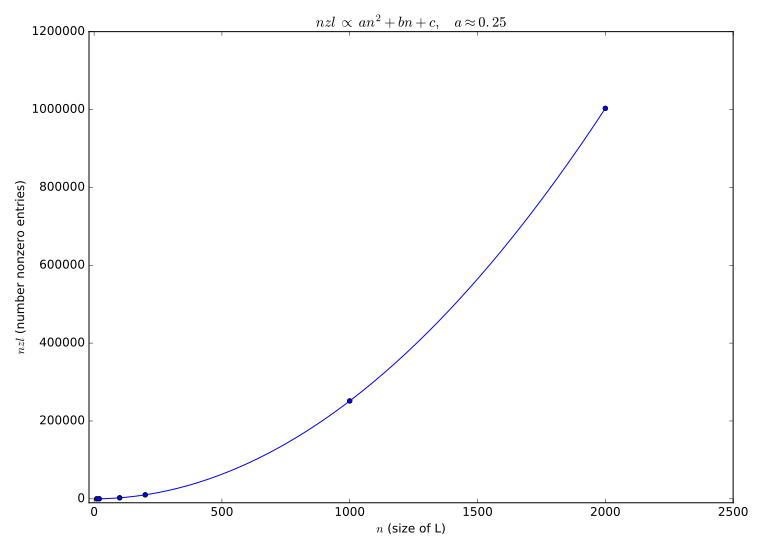
\includegraphics[width=\linewidth]{hw4_1b.png}
        \caption{Relationship between size of system $n$ and number of nonzero elements in Cholesky factor.
        The relationship was found to be quadratic with leading coefficient $a \approx 0.25$.}
    \end{figure}
    Output of spy(L) for $n=2000$:
    \begin{figure}
    \includegraphics[width=\linewidth]{hw4_spy.png}
    \caption{A visualization of nonzero elements of the cholesky factor $L$ when $n=1000$ of the matrix A}
\end{figure}
\end{enumerate}
\end{prob}
\end{document}
